
C++类通常是“空的”,内部表示在运行时不需要内存位。对于只包含类型成员、非虚函数成员和静态数据成员的类,通常是这样。另一方面,非静态数据成员、虚函数和虚基类在运行时确实需要一些内存。

即使是空类,其大小也是非零的。如果想验证这一点,可以试试下面的代码:

\hspace*{\fill} \\ %插入空行
\noindent
\textit{inherit/empty.cpp}
\begin{lstlisting}[style=styleCXX]
#include <iostream>

class EmptyClass {
};

int main()
{
	std::cout << "sizeof(EmptyClass): " << sizeof(EmptyClass) << ’\n’;
}
\end{lstlisting}

对于多数平台,这个程序将输出1作为EmptyClass的大小。一些系统对类类型有更严格的对齐要求,可能会打印另一个小整数(通常为4)。

\subsubsubsection{21.1.1\hspace{0.2cm}结构布置原则}

C++的设计者有各种理由来避免零大小的类。例如,一个由零大小类组成的数组的大小应该也为零,但是指针算法的属性将不再适用。假设ZeroSizedT是一个零大小的类型:

\begin{lstlisting}[style=styleCXX]
ZeroSizedT z[10];
...
&z[i] - &z[j] // compute distance between pointers/addresses
\end{lstlisting}

通常,前一个示例中的差异是通过两个地址之间的字节数,除以它所指向的类型的大小得到的,但当该大小为零时,这显然不令人满意。

然而,即使在C++中没有零大小的类型,C++标准指定一个空类作为基类时,不需要为它分配空间,只要它不会分配到与另一个相同类型对象或子对象相同地址中即可。我们通过一些示例来阐明这个空基类优化(EBCO)在实践中的含义。考虑以下代码:

\hspace*{\fill} \\ %插入空行
\noindent
\textit{inherit/ebco1.cpp}
\begin{lstlisting}[style=styleCXX]
#include <iostream>

class Empty {
	using Int = int; // type alias members don’t make a class nonempty
};

class EmptyToo : public Empty {
};

class EmptyThree : public EmptyToo {
};

int main()
{
	std::cout << "sizeof(Empty): " << sizeof(Empty) << ’\n’;
	std::cout << "sizeof(EmptyToo): " << sizeof(EmptyToo) << ’\n’;
	std::cout << "sizeof(EmptyThree): " << sizeof(EmptyThree) << ’\n’;
}
\end{lstlisting}

如果编译器实现了EBCO,将为每个类打印相同的大小,但这些类的大小都不是0(参见图21.1)。在类EmptyToo中,类Empty没有被赋予空间。还要注意,优化过的空基类(没有其他基类)的空类也是空的。这解释了为什么类EmptyThree也可以具有与类Empty相同的大小。如果编译器没有实现EBCO,将输出不同的大小(参见图21.2)。

\begin{center}
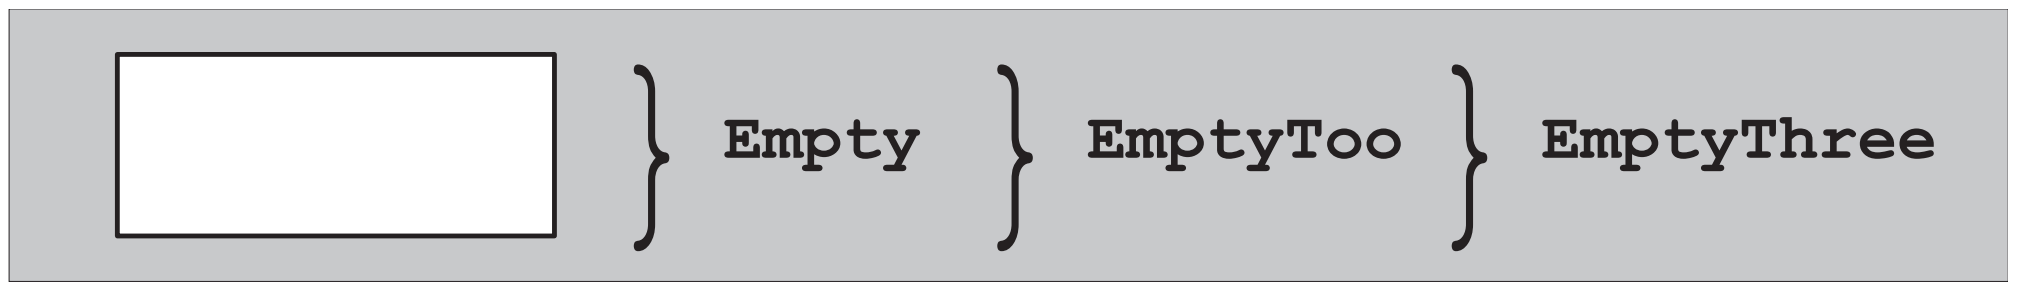
\includegraphics[width=0.8\textwidth]{content/3/chapter21/images/1.png} \\
图21.1. EmptyThree的结构,由实现EBCO的编译器
\end{center}

\begin{center}
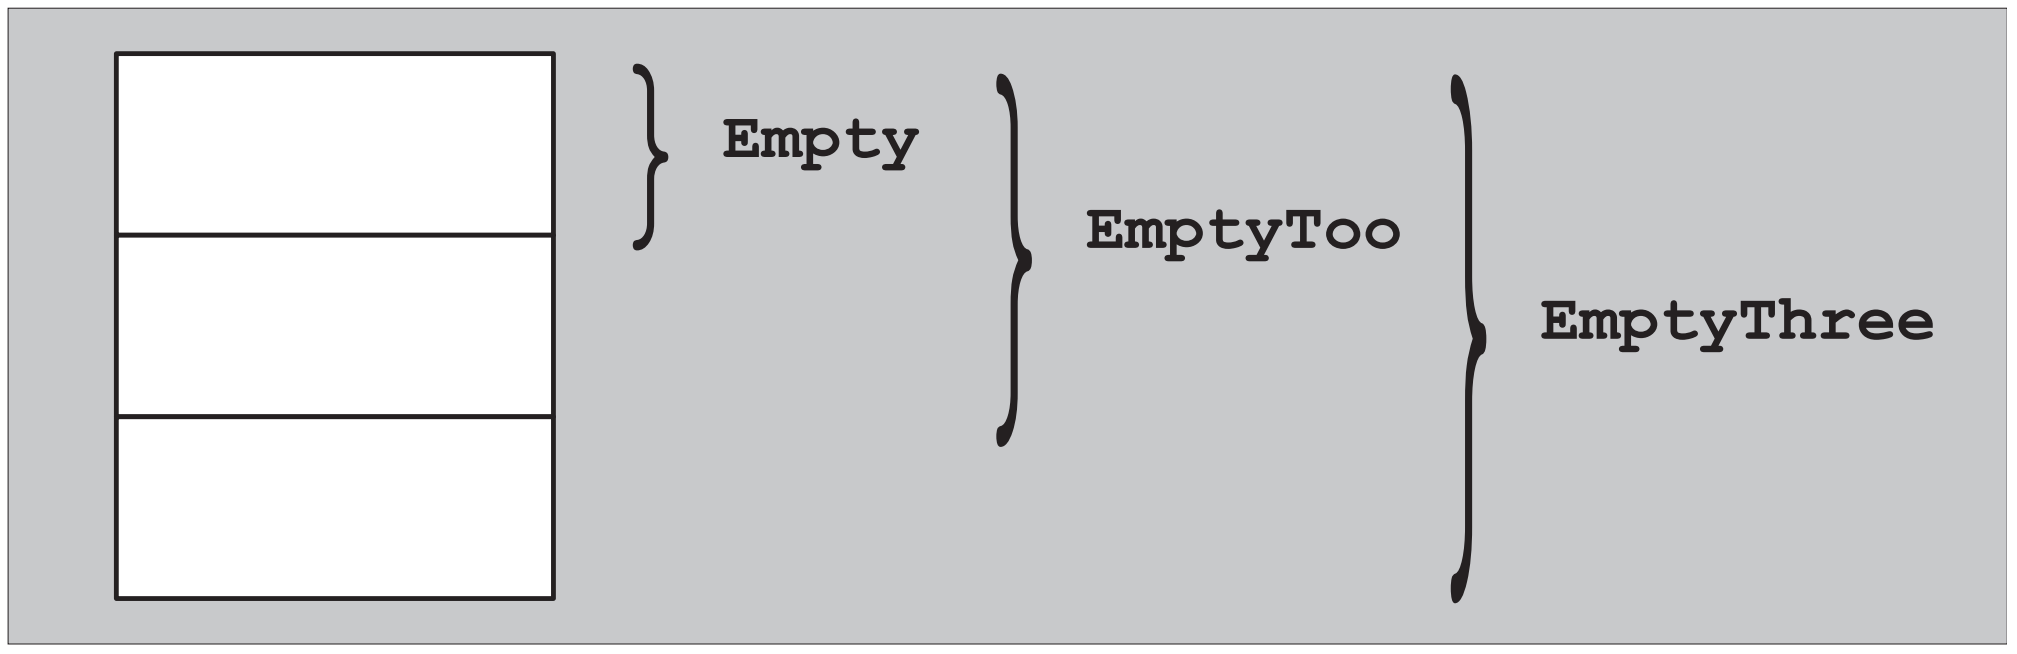
\includegraphics[width=0.8\textwidth]{content/3/chapter21/images/2.png} \\
图21.2. EmptyThree的结构,由未实现EBCO的编译器
\end{center}

考虑一个遇到EBCO约束的情况:

\hspace*{\fill} \\ %插入空行
\noindent
\textit{inherit/ebco2.cpp}
\begin{lstlisting}[style=styleCXX]
#include <iostream>

class Empty {
	using Int = int; // type alias members don’t make a class nonempty
};

class EmptyToo : public Empty {
};

class NonEmpty : public Empty, public EmptyToo {
};

int main()
{
	std::cout << "sizeof(Empty): " << sizeof(Empty) << ’\n’;
	std::cout << "sizeof(EmptyToo): " << sizeof(EmptyToo) << ’\n’;
	std::cout << "sizeof(NonEmpty): " << sizeof(NonEmpty) << ’\n’;
}
\end{lstlisting}

NonEmpty类不是一个空类!它没有任何成员,基类也没有。但是,NonEmpty的基类Empty和EmptyToo不能分配到相同的地址,这将导致EmptyToo的基类Empty与NonEmpty的基类Empty位于相同的地址。换句话说,相同类型的两个子对象将以相同的偏移量结束,而这是C++的对象布局规则不允许的。可以想象,Empty基子对象中的一个放置在偏移量“0字节”处,另一个放置在偏移量“1字节”处,但是完整的NonEmpty对象仍然不能有1字节的大小,因为在两个NonEmpty对象的数组中,第一个元素的Empty子对象不能与第二个元素的Empty子对象在同一地址(参见图21.3)。

\begin{center}
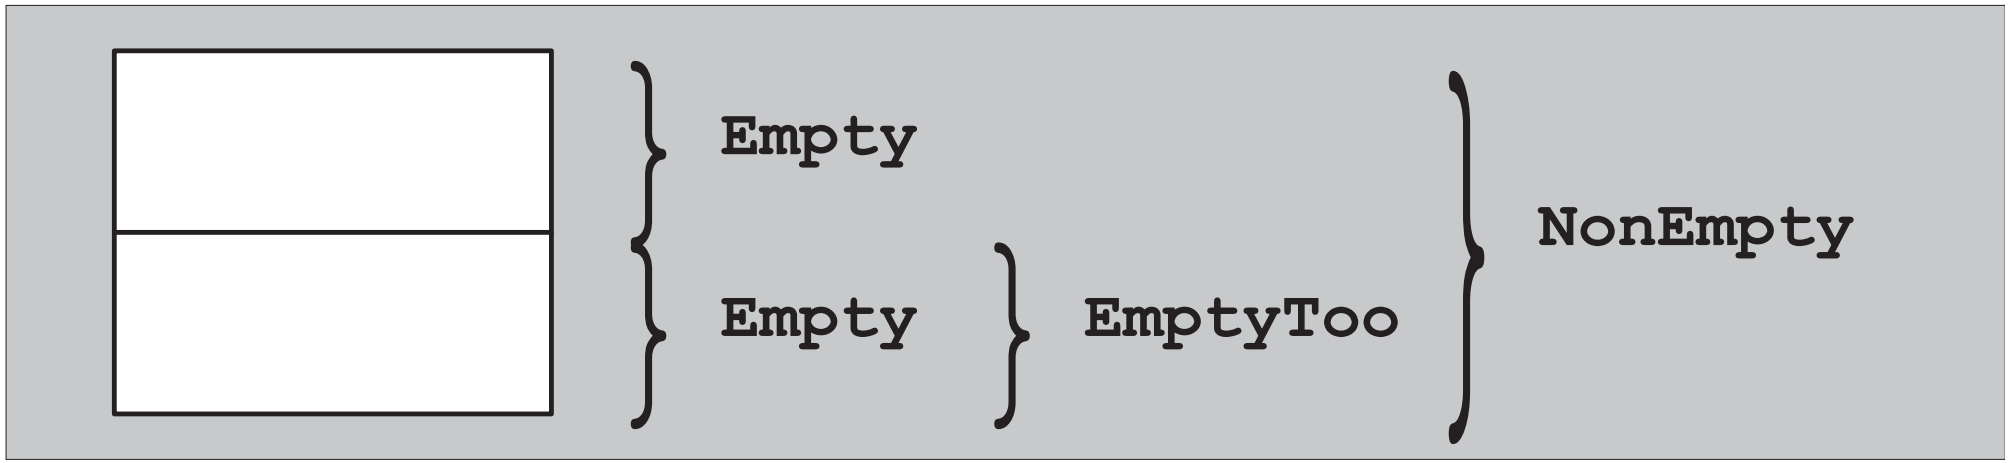
\includegraphics[width=0.8\textwidth]{content/3/chapter21/images/3.png} \\
图21.3. 实现EBCO的编译器的非空结构
\end{center}

对EBCO进行约束的基本原理源于这样一个事实,即能够比较两个指针是否指向同一个对象。因为指针在内部总是表示为地址,必须确保两个不同的地址(即指针值)对应两个不同的对象。

这个限制看起来可能不重要,但在实践中,经常会遇到这种情况,因为许多类倾向于使用一小组定义了一些常见类型别名的空类继承。当此类中的两个子对象同时用于同一完整对象时,就抑制了优化。

即使有这个约束,EBCO仍然是模板库的重要优化,因为许多技术依赖于基类引入,只是为了引入新的类型别名或提供额外的功能,而不添加新数据。

\subsubsubsection{21.1.2\hspace{0.2cm}基类的成员}

EBCO对于数据成员没有同等的功能,因为(在其他方面)会在成员指针的表示方面产生一些问题。因此,有时需要将认为是成员变量的东西实现为(私有)基类。然而,这很有挑战性。

这个问题在模板上下文中最有趣,因为模板参数经常使用空类类型替换,但我们不能依赖于此规则。如果对模板类型参数一无所知,就不能使用EBCO。考虑一下下面这个例子:

\begin{lstlisting}[style=styleCXX]
template<typename T1, typename T2>
class MyClass {
	private:
	T1 a;
	T2 b;
	...
};
\end{lstlisting}

完全有可能使用空类类型替代一个或两个模板参数。若是这样,那么MyClass<T1,T2>的表示可能是次优的,并且可能为每个MyClass<T1,T2>的实例浪费一个字符的内存。

可以通过将模板参数设置为基类来避免这种情况的发生:

\begin{lstlisting}[style=styleCXX]
template<typename T1, typename T2>
class MyClass : private T1, private T2 {
};
\end{lstlisting}

然而,这种简单的替代方法也存在一些问题:

\begin{itemize}
\item 
当使用非类类型或联合类型替代T1或T2时,这种方式就不起作用。

\item 
当两个参数替换为相同类型时,也不起作用(尽管这可以通过添加另一层继承来解决)。

\item 
类可以是final类,在这种情况下,试图对它进行继承将导致编译错误。
\end{itemize}

即使圆满地解决了这些问题,另一个严重的问题仍然存在:添加基类会从根本上修类的接口。对于MyClass类,这似乎不太重要,因为要影响的接口元素很少,但在后面会看到,从模板参数继承可以影响成员函数是否为虚函数。显然,这种使用EBCO的方法存在各种麻烦。

当模板参数只能由类类型替换,且类模板的另一个成员可用时,可以设计一种更实用的工具。主要思想是使用EBCO将可能为空的类型参数与其他成员“合并”。例如,

\begin{lstlisting}[style=styleCXX]
template<typename CustomClass>
class Optimizable {
	private:
	CustomClass info; // might be empty
	void* storage;
	...
};
\end{lstlisting}

模板实现者会使用以下语句:

\begin{lstlisting}[style=styleCXX]
template<typename CustomClass>
class Optimizable {
	private:
	BaseMemberPair<CustomClass, void*> info_and_storage;
	...
};
\end{lstlisting}

即使没有看到模板BaseMemberPair的实现,这样也会使Optimizable的实现更加冗长。然而,各种模板库实现者都说,性能的提高(对于他们库的客户端来说)证明了增加复杂性的合理性。我们将在第25.1.1节中讨论元组存储时,进一步探讨这种习惯性用法。

BaseMemberPair的实现可以很紧凑:

\hspace*{\fill} \\ %插入空行
\noindent
\textit{inherit/basememberpair.hpp}
\begin{lstlisting}[style=styleCXX]
#ifndef BASE_MEMBER_PAIR_HPP
#define BASE_MEMBER_PAIR_HPP

template<typename Base, typename Member>
class BaseMemberPair : private Base {
	private:
	Member mem;
	
	public:
	// constructor
	BaseMemberPair (Base const & b, Member const & m)
	: Base(b), mem(m) {
	}
	// access base class data via first()
	Base const& base() const {
		return static_cast<Base const&>(*this);
	}
	Base& base() {
		return static_cast<Base&>(*this);
	}
	// access member data via second()
	Member const& member() const {
		return this->mem;
	}
	Member& member() {
		return this->mem;
	}
};

#endif // BASE_MEMBER_PAIR_HPP
\end{lstlisting}

实现需要使用成员函数base()和member()来访问封装(可能经过存储优化)的数据成员。





























